\subsection{Activity}

L'\textbf{Activity Diagram} serve a descrivere logica procedurale, processi di business e workflow. In UML 1.0 era un caso particolare degli \textit{State Diagram}. Sono simili ai \textit{flowchart} ma supportano la rappresentazione di elaborazione parallela.

\paragraph{Descrizione} L'esecuzione inizia in corrispondenza del \textbf{nodo iniziale} (pallino nero) e si conclude al \textbf{nodo finale} (pallino bianco). I \textbf{nodi attività} (rettangolo a bordi smussati) descrivono le azioni da svolgere. I nodi sono collegati da \textbf{archi}; un percorso dal nodo iniziale al nodo finale rappresenta un \textbf{flusso di attività} (\textit{activity flow}). Per semplicità è possibile usare coppie di \textbf{connettori} con la stessa \textit{etichetta} al posto degli archi. I flussi possono essere:
\begin{itemize}
    \item \textbf{alternativi}: rombi con un solo arco entrante e più archi uscenti (\textbf{decision}) aventi ciascuno un proprio valore di \textit{guardia} (che ne decide l'esecuzione). I flussi confluiscono in un rombo con molti archi entranti ed un solo arco uscente (\textbf{merge}).
    \item \textbf{paralleli}: si diramano da una barra con un solo arco entrante e più archi uscenti (\textbf{fork}). I flussi possono essere eseguiti in maniera concorrente e confluiscono in una barra avente molti archi entranti ed un arco uscente (\textbf{join}).
\end{itemize}
All'interno di un nodo attività si può inserire un'icona a forma di rastrello che indica che l'attività è un flusso specificato da un ulteriore activity diagram di livello inferiore (diagramma secondario).

\begin{figure}[H]
    \subfloat[Semplice diagramma di esempio]{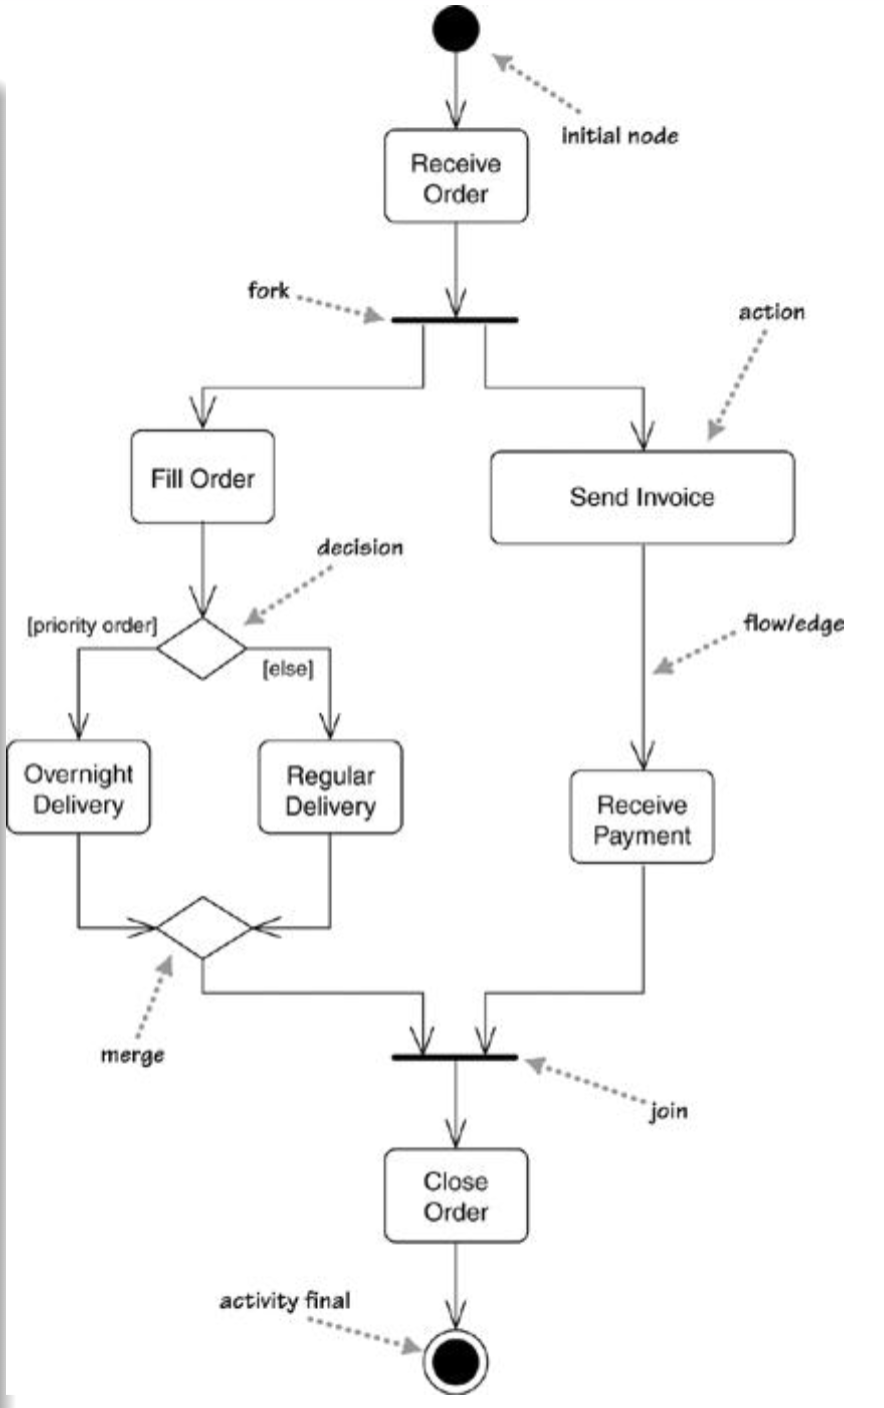
\includegraphics[width=0.4\linewidth]{assets/UML/activity/activity-1.png}}
    \hfill
    \subfloat[Esempio di partizione]{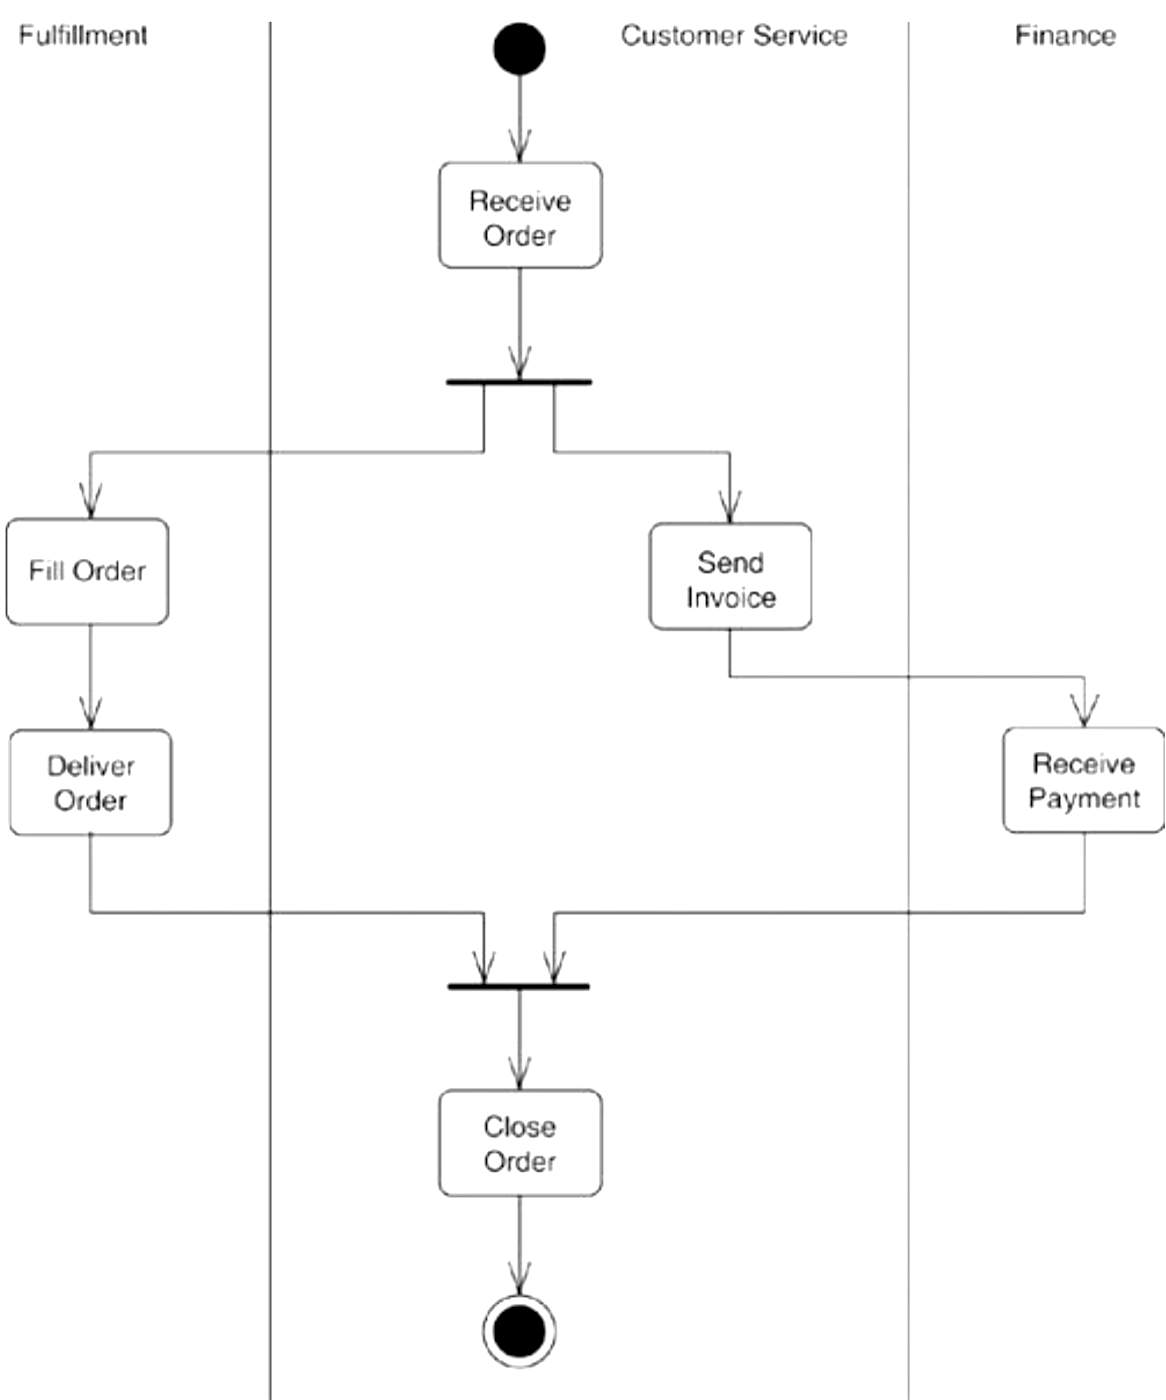
\includegraphics[width=0.55\linewidth]{assets/UML/activity/activity-3.png}}
\end{figure}

\paragraph{Specifiche di Join} Le operazioni di join operano la “sincronizzazione” tra flussi. È possibile introdurre una condizione booleana per la quale si può proseguire (viene rispettata) solo se tutti i flussi paralleli hanno terminato la loro esecuzione.

\paragraph{Partizioni} L'activity diagram può essere partizionato sulla base delle \textit{tipologie di attività} o dell'\textit{entità} adibita a svolgerle. Sono rappresentate tramite un'icona a \textit{rastrello}. Una determinata azione può essere implementata da un metodo; in tal caso si usa la sintassi “nomeClasse::nomeMetodo”. In un diagramma partizionato sono presenti delle \textbf{swim lane}: linee verticali che consentono di separare le competenze.

\begin{figure}[H]
    \subfloat[Diagramma secondario]{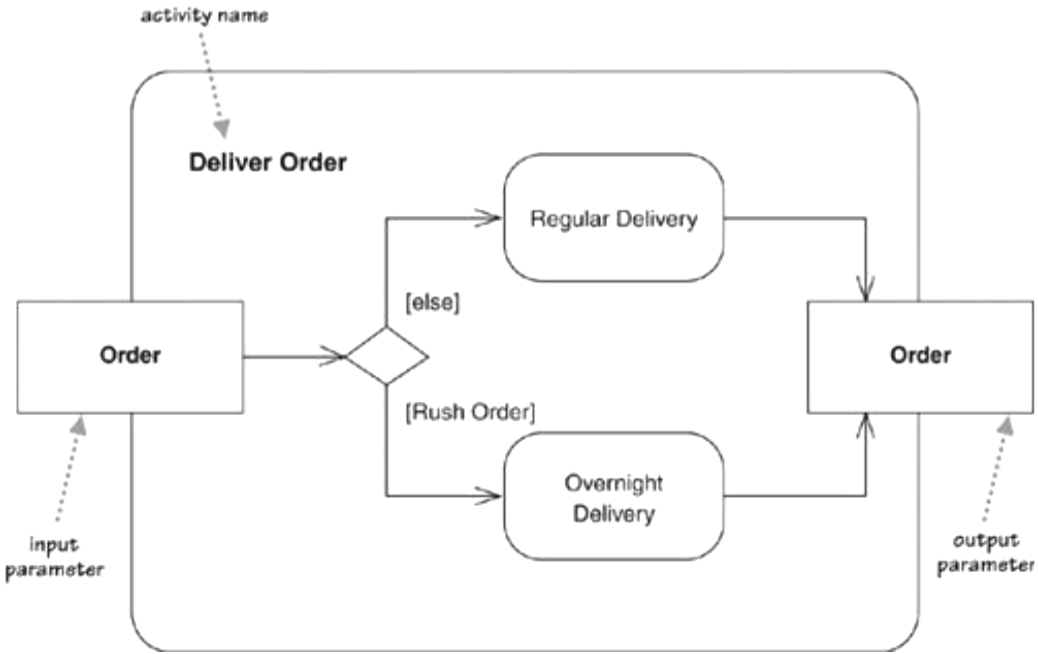
\includegraphics[width=0.55\linewidth]{assets/UML/activity/activity-2.png}}
    \hfill
    \subfloat[Utilizzo di flussi e connettori]{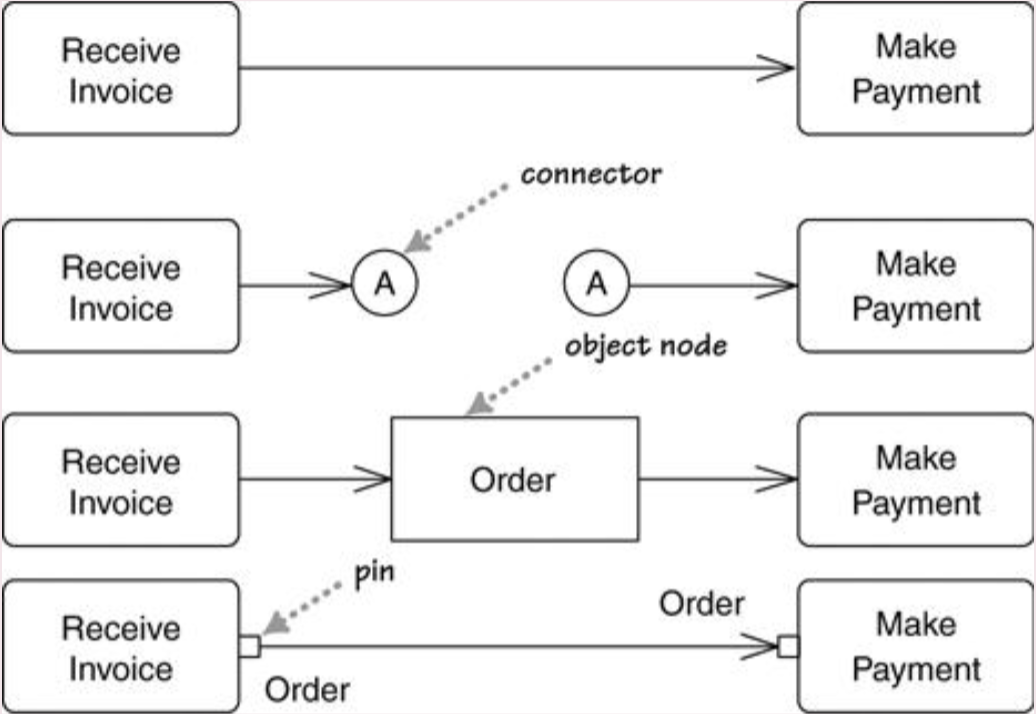
\includegraphics[width=0.4\linewidth]{assets/UML/activity/activity-4.png}}
\end{figure}

\newpage
\paragraph{Segnali} Eventi che il sistema può ricevere o generare da/verso l'esterno. Possono essere \textbf{temporali} (clessidre) o \textbf{personali} (generati da azioni, ad esempio).

\begin{figure}[H]
    \subfloat{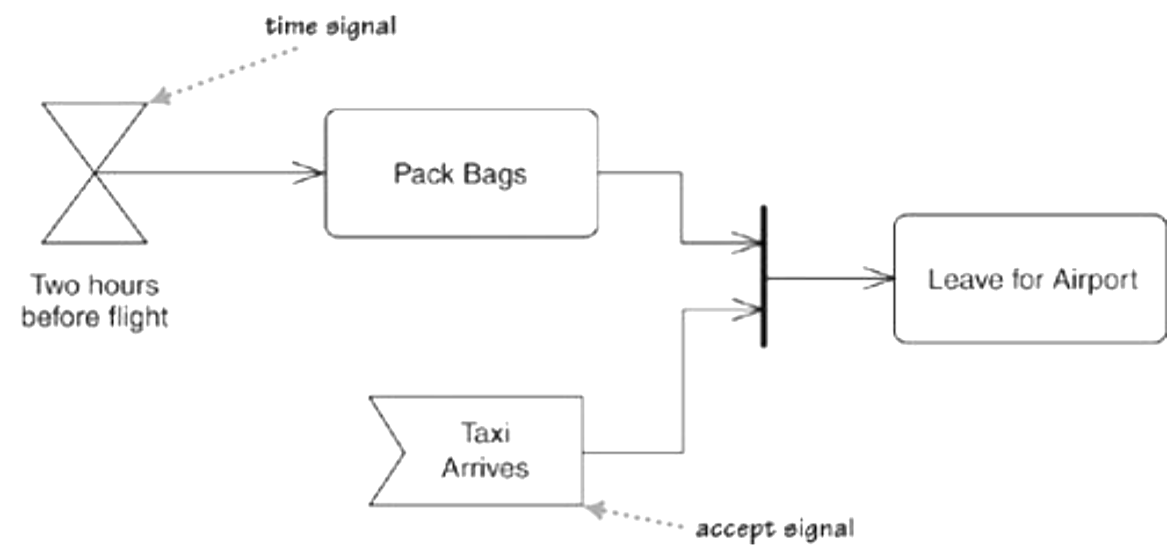
\includegraphics[width=0.455\linewidth]{assets/UML/activity/activity-6.png}}
    \hfill
    \subfloat{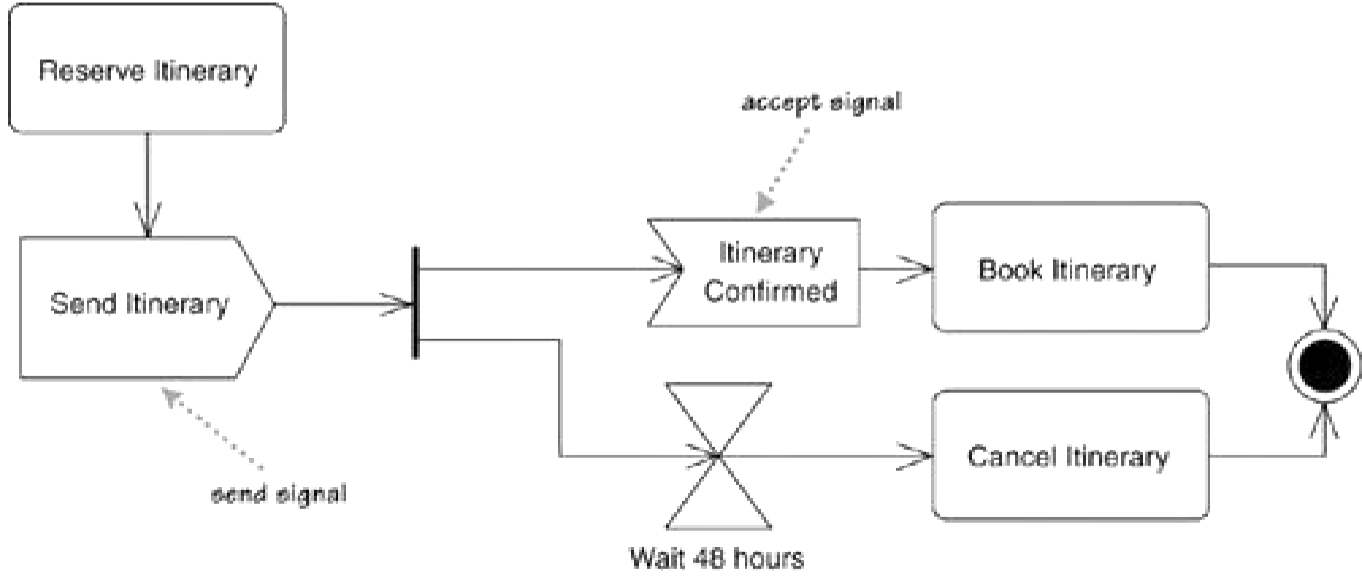
\includegraphics[width=0.5\linewidth]{assets/UML/activity/activity-5.png}}
    \caption{Esempi di utilizzo di \textbf{segnali}}
\end{figure}

\begin{figure}[H]
    \centering
    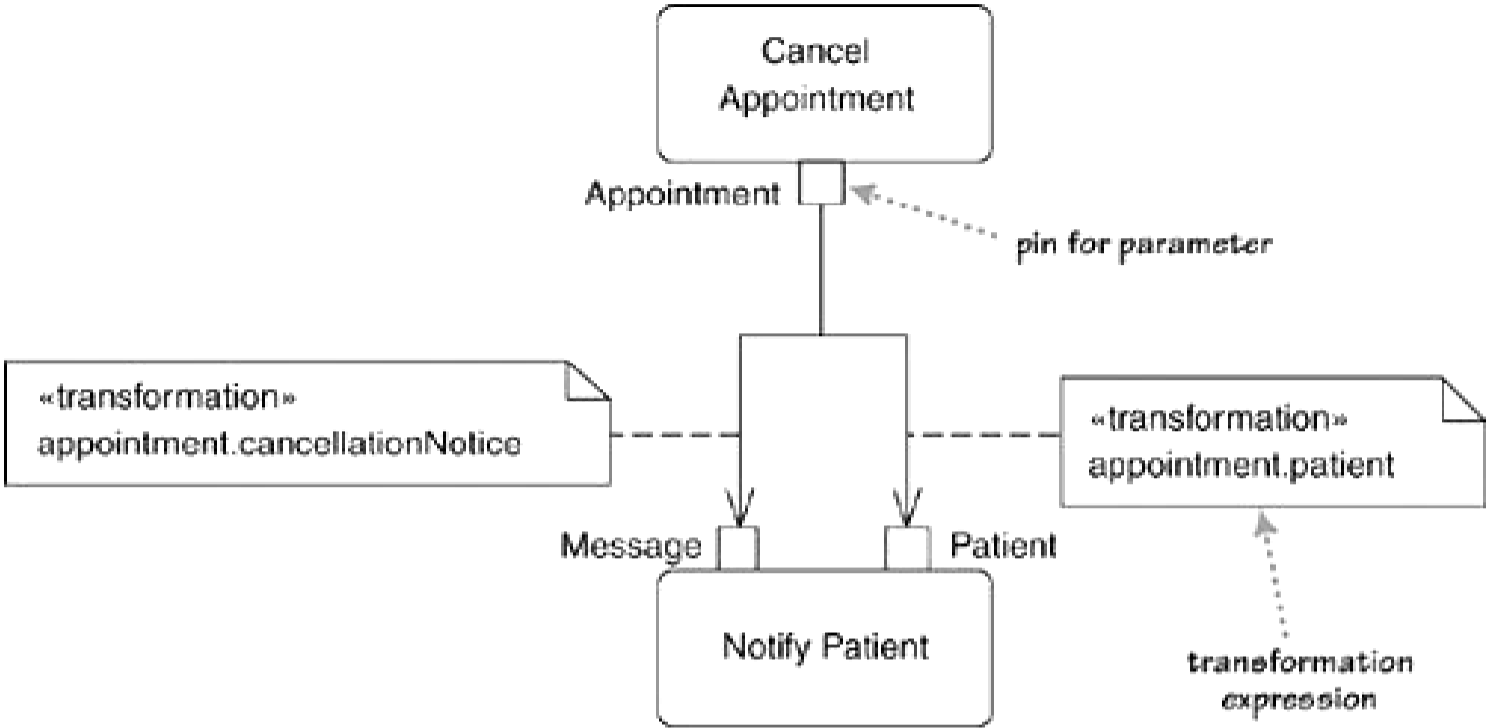
\includegraphics[width=0.75\linewidth]{assets/UML/activity/activity-7.png}
    \caption{I \textbf{pin} consentono di identificare oggetti in input/output per le attività. Le \textbf{trasformazioni} mostrano le modifiche subite dagli oggetti nelle attività.}
\end{figure}

\paragraph{Regione di espansione} Insieme di attività che devono essere eseguite per ogni elemento di una lista di oggetti in ingresso. Restituiscono in output un'altra lista di oggetti.

\begin{figure}[H]
    \centering
    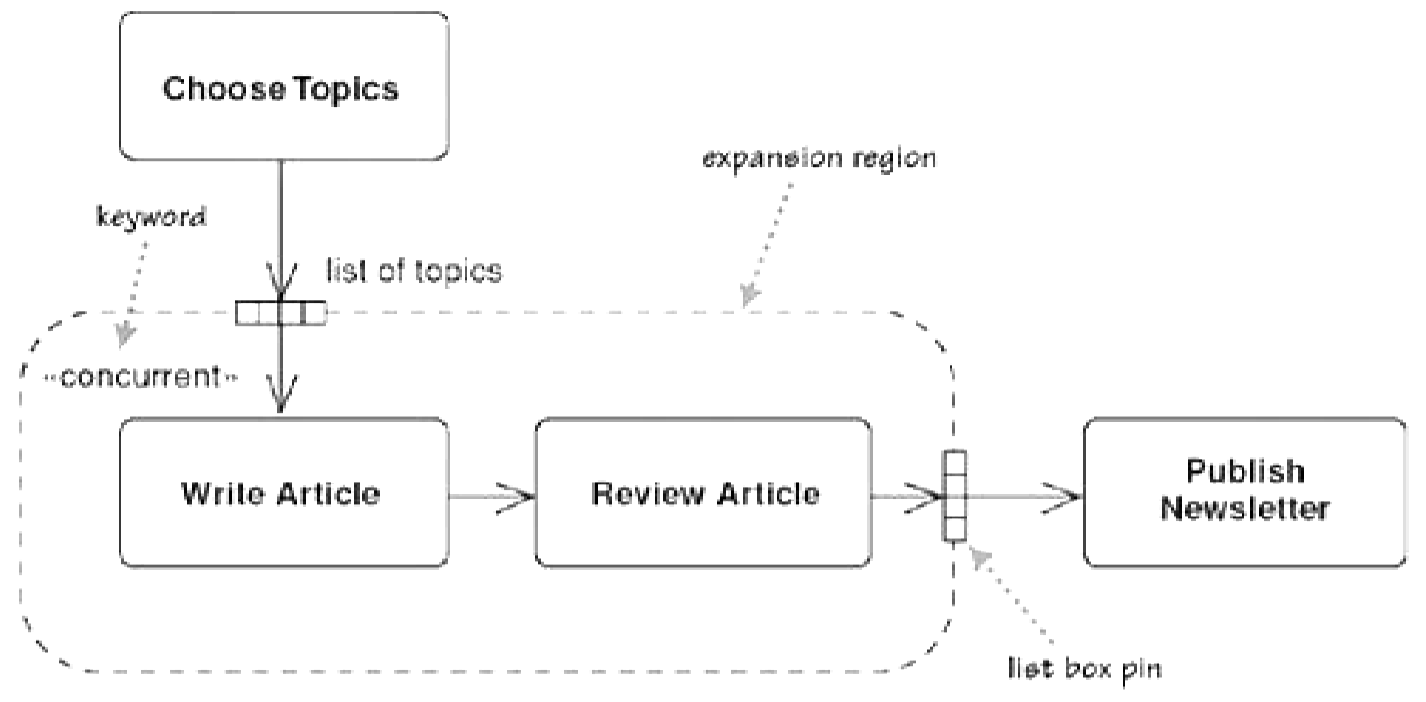
\includegraphics[width=0.8\linewidth]{assets/UML/activity/activity-8.png}
    \caption{Esempio di utilizzo di \textbf{regioni di espansione}}
\end{figure}

\begin{figure}[H]
    \centering
    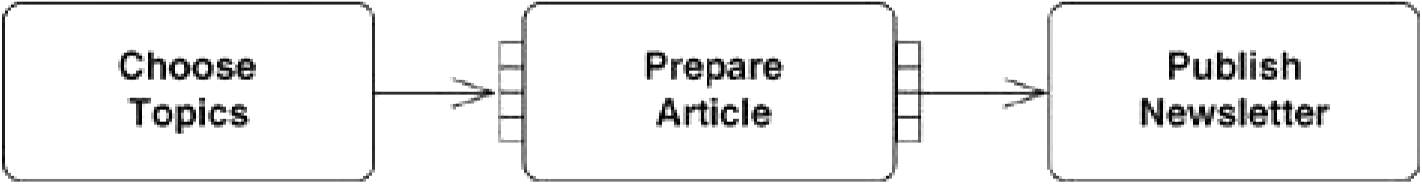
\includegraphics[width=0.8\linewidth]{assets/UML/activity/activity-9.png}
    \caption{Diagramma semplificato risultante a seguito della specifica della regione di espansione}
\end{figure}

\newpage